%&pdflatex
\documentclass[11pt, a4paper]{article}
\usepackage{graphicx}
\usepackage{amsmath}
\usepackage{listings}
\usepackage{minted}
\usepackage{float}

\title{EE2703 Applied Programming Lab - \\Assignment No 5}
\author{
  \textbf{Name}: Abishek S\\
  \textbf{Roll Number}: EE18B001
}\date{\today}
\begin{document}
		
\maketitle 
\section{Abstract}
The goal of this assignment is the following :
\begin{itemize}
\item To plot contour and 3-D plots.
\item To solve 2-D Laplace equation in an iterative manner.
\item To use vectorized code in Python.
\item To observe the variation of error with iteration.
\end{itemize}
\usemintedstyle{manni}

\section{Assignment}
For DC current, the 2-D Laplace equation is :
\begin{equation}\label{eq:1}
\nabla^2\phi = 0
\end{equation}
\begin{center}
\textbf{OR}
\end{center}
\begin{equation}\label{eq:2}
\frac{\partial^2\phi}{\partial x^2} + \frac{\partial^2\phi}{\partial y^2} = 0
\end{equation}
\\
\subsection{Setting the parameters and making contour plot of \\Potential }
Importing the standard libraries
\begin{minted}[mathescape,escapeinside = ||,tabsize = 4]{python3}
import pylab as pl
import mpl_toolkits.mplot3d.axes3d as p3
import argparse
import numpy as np
from scipy.linalg import lstsq
import sys
import matplotlib
\end{minted}
Using argparse, getting optional inputs for Nx,Ny,radius and Niter from the command line and also defined their default values.
\begin{minted}[tabsize = 4]{python3}
parser = argparse.ArgumentParser(description='Defining Parameters')
parser.add_argument('-Nx',dest='Nx',type=int,default=25,help = 'Size along x')
parser.add_argument('-Ny',dest='Ny',type=int,default=25,help = 'Size along y')
parser.add_argument('-r',dest='radius',type=int,default=8,
								help = 'Radius of central lead')
parser.add_argument('-Ni',dest='Niter',type=int,default=1500,
								help = 'Number of interations to perform')
args = parser.parse_args()
Nx,Ny,Niter,radius = args.Nx,args.Ny,args.Niter,args.radius
\end{minted}
We define a plotting function to simplify our code.
\begin{minted}[tabsize = 4]{python3}
def PLOT(x,y,fig_no = 0,label_x = r'$\rightarrow$',label_y = r'$\rightarrow$',
		fn = pl.plot,\\arg3 = 'b-',title = "Plot",grids = True,
		cmap = matplotlib.cm.jet,label = ''):
	pl.figure(fig_no)
	pl.grid(grids)
	if fn == pl.contourf:
		fn(x,y,arg3,cmap = cmap)
		pl.colorbar()
	else:
		if label == '':
			fn(x,y,arg3)
		else:
			fn(x,y,arg3,label = label)
	pl.xlabel(label_x)
	pl.ylabel(label_y)
	pl.title(title)
\end{minted}
We allocate and initialize the potential array.
\begin{minted}[tabsize = 4]{python3}
Phi = np.zeros(shape = (Ny,Nx))
x = np.linspace(-0.5,0.5,Nx)
y = np.linspace(-0.5,0.5,Ny)
Y,X = np.meshgrid(y,x)
\end{minted}
We find the points with in the radius of 0.35 cm from the center in 1cm x 1cm grid and plot the contour of the potential.
\begin{minted}[tabsize = 4]{python3}
ii = np.where(X*X + Y*Y <= 0.35*0.35)
Phi[ii] = 1

PLOT(x,y,1,"X-axis","Y-axis",pl.contourf,Phi,"Contour Plot of Potential",
		True,matplotlib.cm.hot)
pl.plot(X[X*X + Y*Y < 0.35*0.35],Y[X*X + Y*Y < 0.35*0.35],'ro',
		label = 'Points with potential 1V')
pl.legend()
pl.show()
\end{minted}

\begin{figure}[H]
   	\centering
   	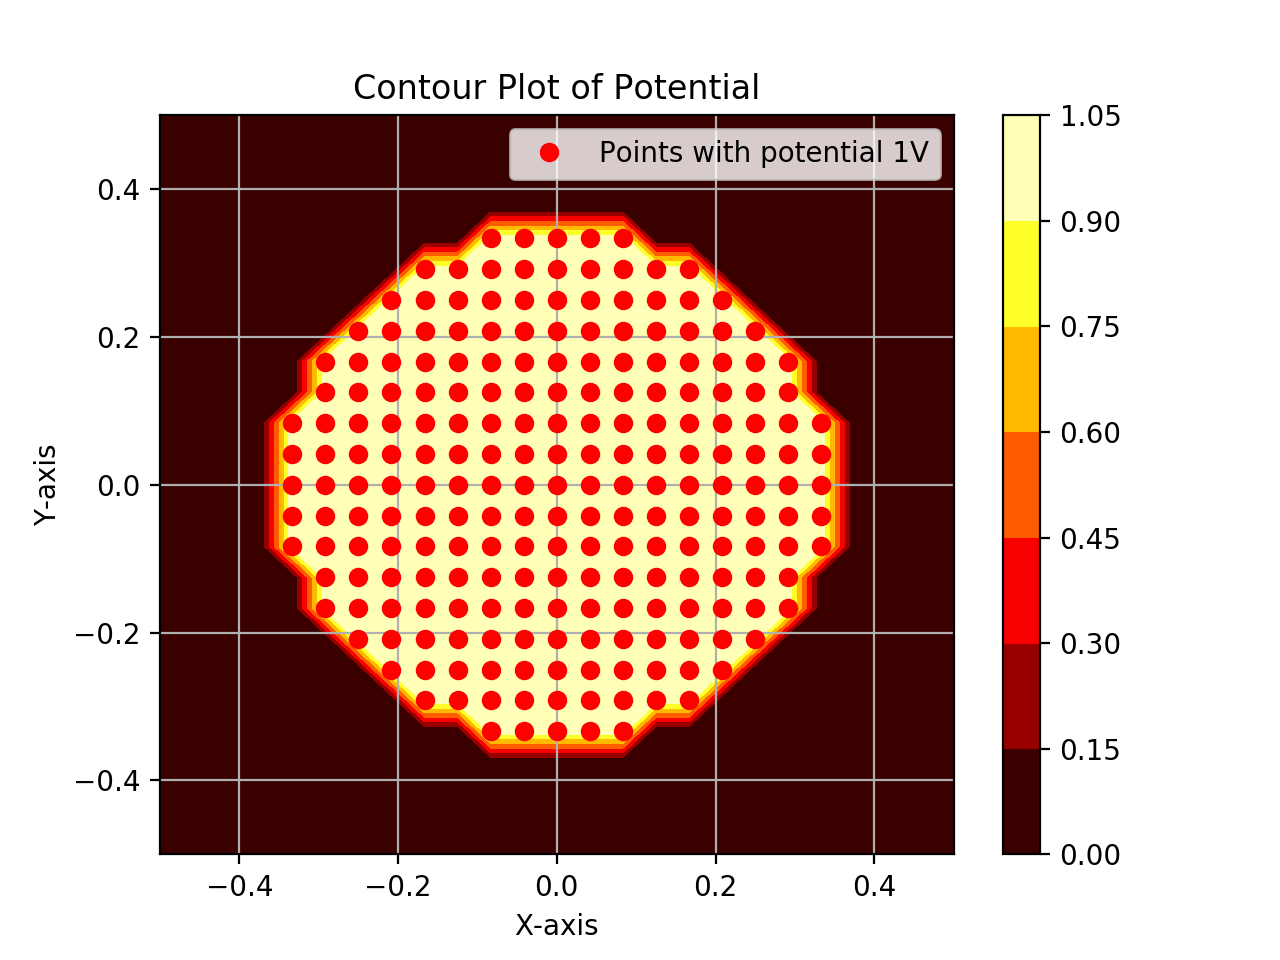
\includegraphics[scale=0.5]{cont_potl_i.png}
   	\label{fig:cont_potl_i}
   	\caption{Contour Plot of Potential}
\end{figure}

\subsection{Solving the 2-D Laplace equation}
We solve the 2-D laplace equation by updating the potential in many iterations so that it converges. This isn't the best approach, but is the easiest to understand and implement, hence we use it.
\\We use the below formula for updating the potential in each iteration : 
\begin{equation} \label{eq:3}
\phi_{i,j} = \frac{\phi_{i+1,j} + \phi_{i-1,j} + \phi_{i,j+1} + \phi_{i,j-1}}{4}
\end{equation}
\begin{minted}[tabsize = 4]{python3}
errors = np.zeros(Niter)
for k in range(Niter):
	oldphi = Phi.copy()
	Phi[1:-1,1:-1] = 0.25*(Phi[1:-1,0:-2]+Phi[1:-1,2:]
							+Phi[0:-2,1:-1]+Phi[2:,1:-1])
	Phi[0,:] = 0
	Phi[1:-1,0] = Phi[1:-1,1]
	Phi[1:-1,-1] = Phi[1:-1,-2]
	Phi[-1,:] = Phi[-2,:]
	Phi[ii] = 1.0
	errors[k] = (abs(Phi-oldphi)).max()
\end{minted}

\subsection{Plotting the Error}
We plot the error vs iteration number- in loglog anf semilog plots.
We notice that the error varies linearly in semilog plot for higher iterations.
\begin{minted}[tabsize = 4]{python3}
#Semilog Plot
PLOT(np.arange(1,Niter+1),errors,2,"Iteration Number","Log of Error",
	fn = pl.semilogy,title='Semilogy Plot of Error vs Iteration Number',
	label = 'Line')
pl.semilogy(np.arange(1,Niter+1,30),errors[0:Niter:30],'yo',label = 'Points')
pl.legend()
pl.show()

#Loglog plot
PLOT(np.arange(1,Niter+1),errors,3,"Log of Iteration Number","Log of Error",
	fn = pl.loglog,title='Loglog Plot of Error vs Iteration Number',
	label = 'Line')
pl.loglog(np.arange(1,Niter+1,30),errors[0:Niter:30],'yo',label = 'Points')
pl.legend()
pl.show()

#Semilog plot after 500 iterations
PLOT(np.arange(500,Niter+1),errors[499:],4,"Iteration Number","Log of Error",
	fn = pl.semilogy,title='Semilogy Plot of Error vs Iteration Number 
	after 500 iterations',label = 'Line')
pl.legend()
pl.show()
\end{minted}

\begin{figure}[H]
   	\centering
   	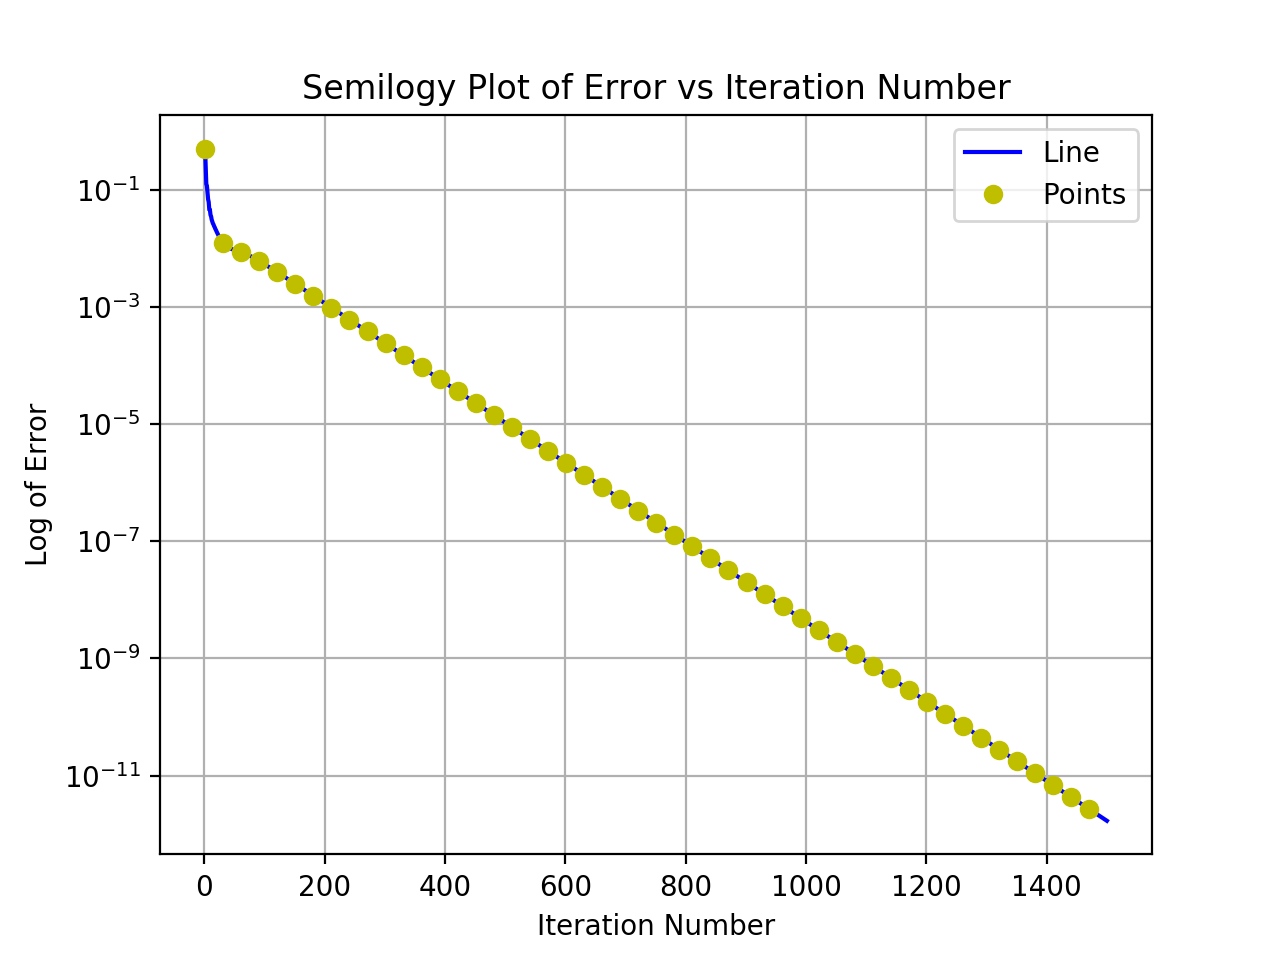
\includegraphics[scale=0.5]{semilog_pt.png}
   	\label{fig:semilog_pt}
   	\caption{Error vs Iteration - Semilog Plot}
\end{figure}
\begin{figure}[H]
   	\centering
   	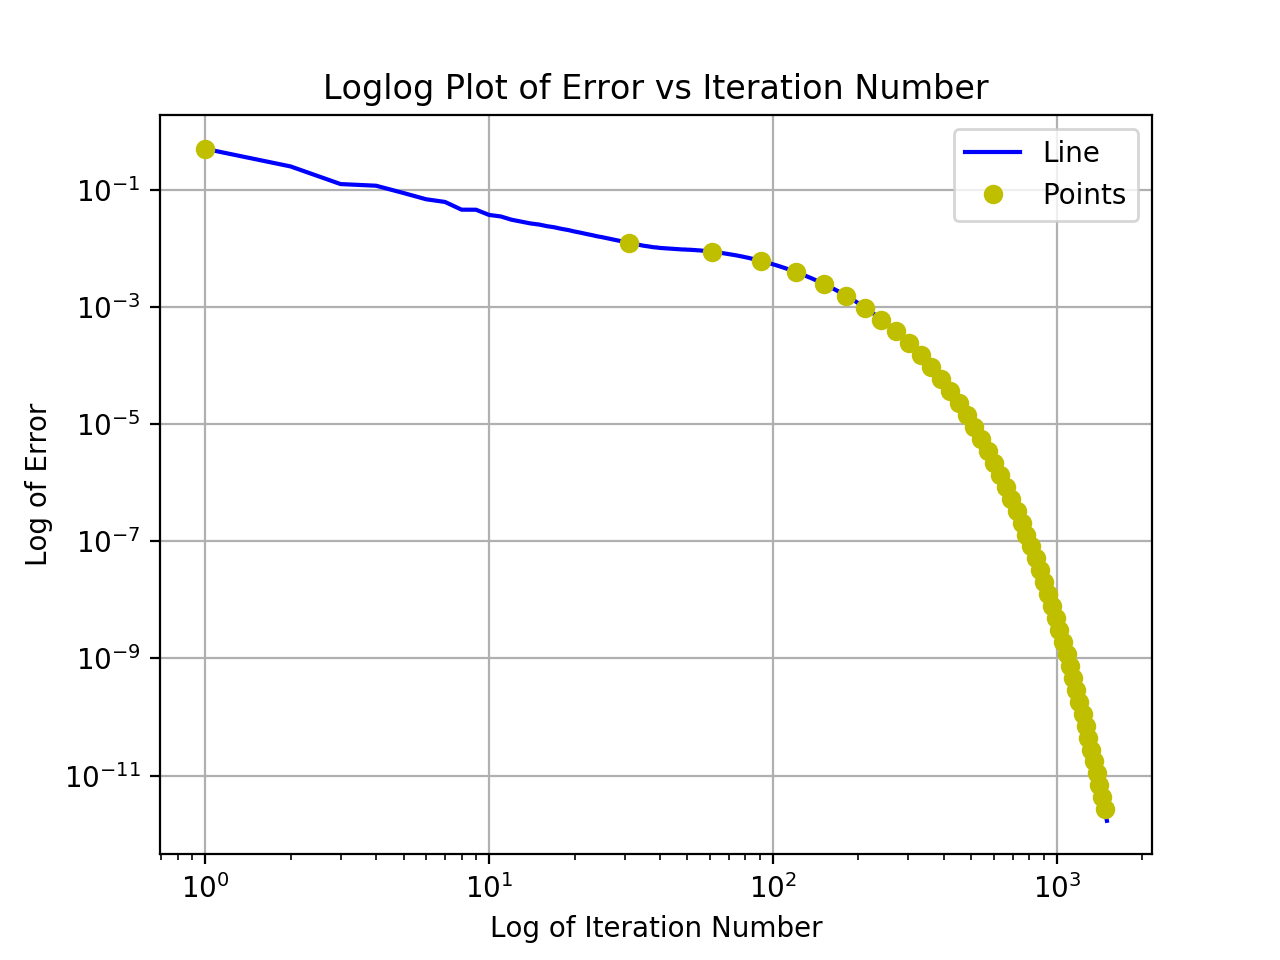
\includegraphics[scale=0.5]{loglog_pt.png}
   	\label{fig:loglog_pt}
   	\caption{Error vs Iteration - Loglog Plot}
\end{figure}
   
\begin{figure}[H]
   	\centering
   	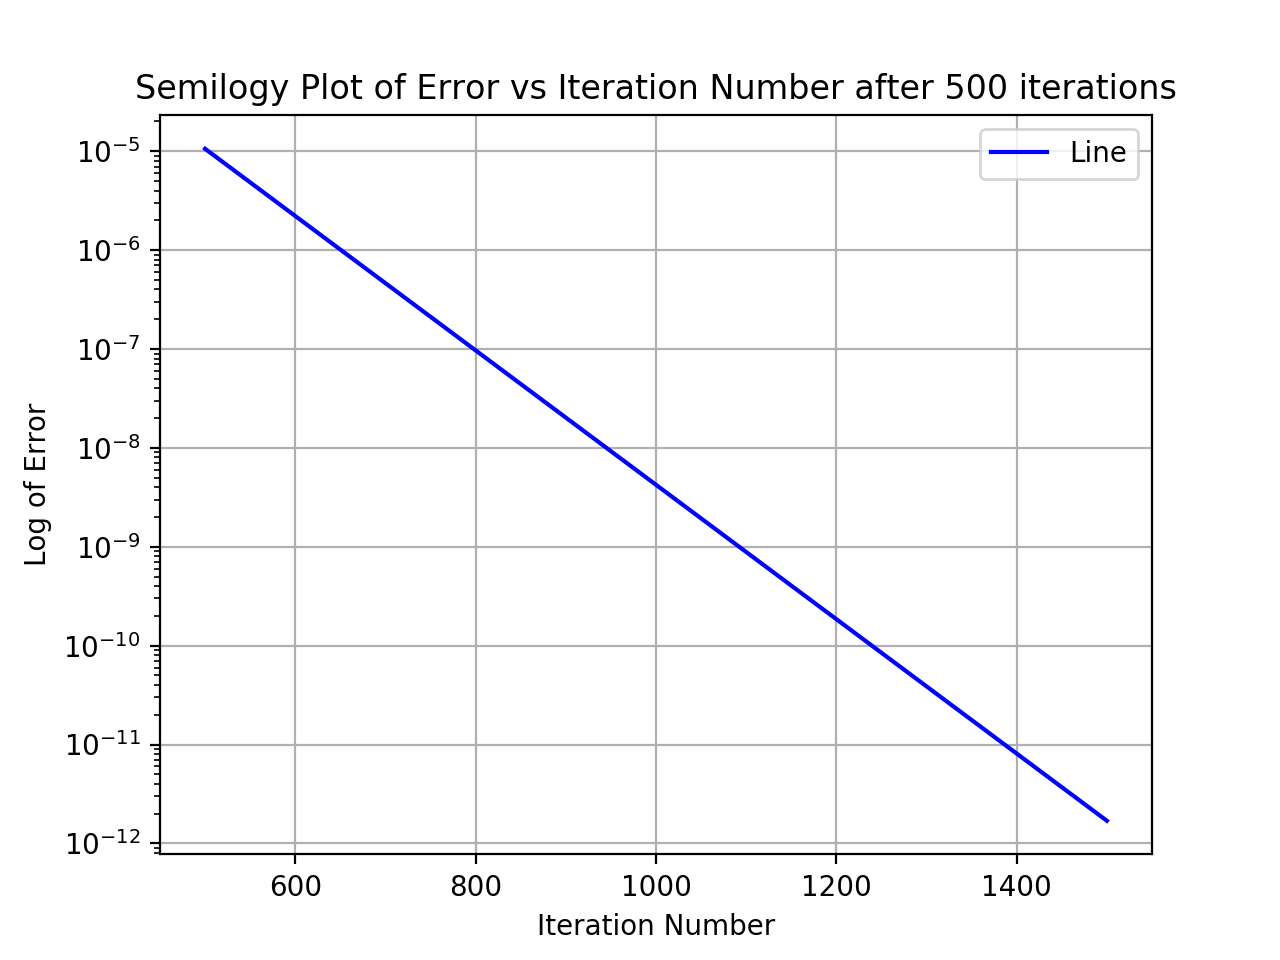
\includegraphics[scale=0.5]{semilog_500.png}
   	\label{fig:semilog_500}
   	\caption{Error vs Iteration for Higher iterations ($>= 500$) - Semilog Plot}
\end{figure}

\subsection{Obtaining a fitting for the Error and plotting it}
We noticed how the error varies linearly with iteration number for higher iterations ($>= 500$).
Thus,  we can assume the error (E) to vary as :
$Ae^{Bk}$\\
where \textbf{A,B} are parameters we need to figure out, and \textbf{k} is the iteration number.
We use Least linear fitting to obtain parameters A and B since taking log of the above equation, we obtain :
\begin{equation}\label{eq:4}
log E = log A + By \\
\end{equation}
We obtain two fittings :\\
\textbf{Fit 1} - Fitting the nearly linear portion of semilog plot ($>= 500$) iterations using :
\begin{equation}\label{eq:5}
\begin{pmatrix}
1 & 500 \\
1 & 501 \\
... & ... \\
1 & 1500 
\end{pmatrix}
\begin{pmatrix}
log A \\
B
\end{pmatrix}
=
\begin{pmatrix}
E_{500} \\
E_{501} \\
... \\
E_{1500}
\end{pmatrix}
\end{equation}
\textbf{Fit 2} - Fitting the entire error vector (for all iterations) using :
\begin{equation}\label{eq:6}
\begin{pmatrix}
1 & 1 \\
1 & 2 \\
... & ... \\
1 & 1500 
\end{pmatrix}
\begin{pmatrix}
log A \\
B
\end{pmatrix}
=
\begin{pmatrix}
E_{1} \\
E_{2} \\
... \\
E_{1500}
\end{pmatrix}
\end{equation}
We plot Fit 1 and Fit 2 along with the original error.
\begin{minted}[tabsize = 4]{python3}
a,b = lstsq(np.c_[np.ones(Niter-499),np.arange(500,Niter+1)],
	np.log(errors[499:]))[0]
a = np.exp(a)
print('The values of A and B for which Ae^(Bk) fits 
	the error after 500 iterations are:')
print(a,b)
lerr = a * np.exp(b*np.arange(500,Niter+1))

A,B = lstsq(np.c_[np.ones(Niter),np.arange(1,Niter+1)],np.log(errors))[0]
A = np.exp(A)
print('The values of A and B for which Ae^(Bk) fits 
	the entire error vector are:')
print(A,B)
err = A * np.exp(B*np.arange(1,Niter+1))

PLOT(np.arange(1,Niter+1),errors,5,"Iteration Number","Log of Error",
	fn = pl.semilogy,arg3 = 'r-',title='Semilogy Plot of Error vs 
	Iteration Number',label = 'Original Errors')
pl.semilogy(np.arange(500,Niter+1),lerr,'b-',
	label = 'Linearly fitted error for >500 iterations (Fit 1)')
pl.semilogy(np.arange(1,Niter+1),err,'g-',
	label = 'Linearly fitted error for entire error vector (Fit 2)')
pl.legend()
pl.show()
\end{minted}
We obtain the parameters \textbf{A,B} for FIt 1 and Fit 2 using least squares approach. 
\begin{figure}[H]
   	\centering
   	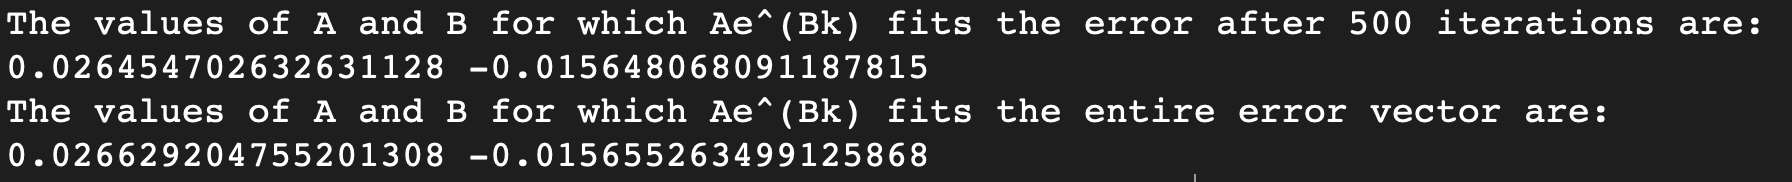
\includegraphics[scale=0.5]{out1.png}
   	\label{fig:out1}
   	\caption{The parameters obtained for Fit 1 and Fit 2}
\end{figure}
We can observe how closer the A's and B's are which happens because the log of error varies non linearly with iteration number only at the beginning for a few iterations, as before updating the potential can be initialised with any values.

\begin{figure}[H]
   	\centering
   	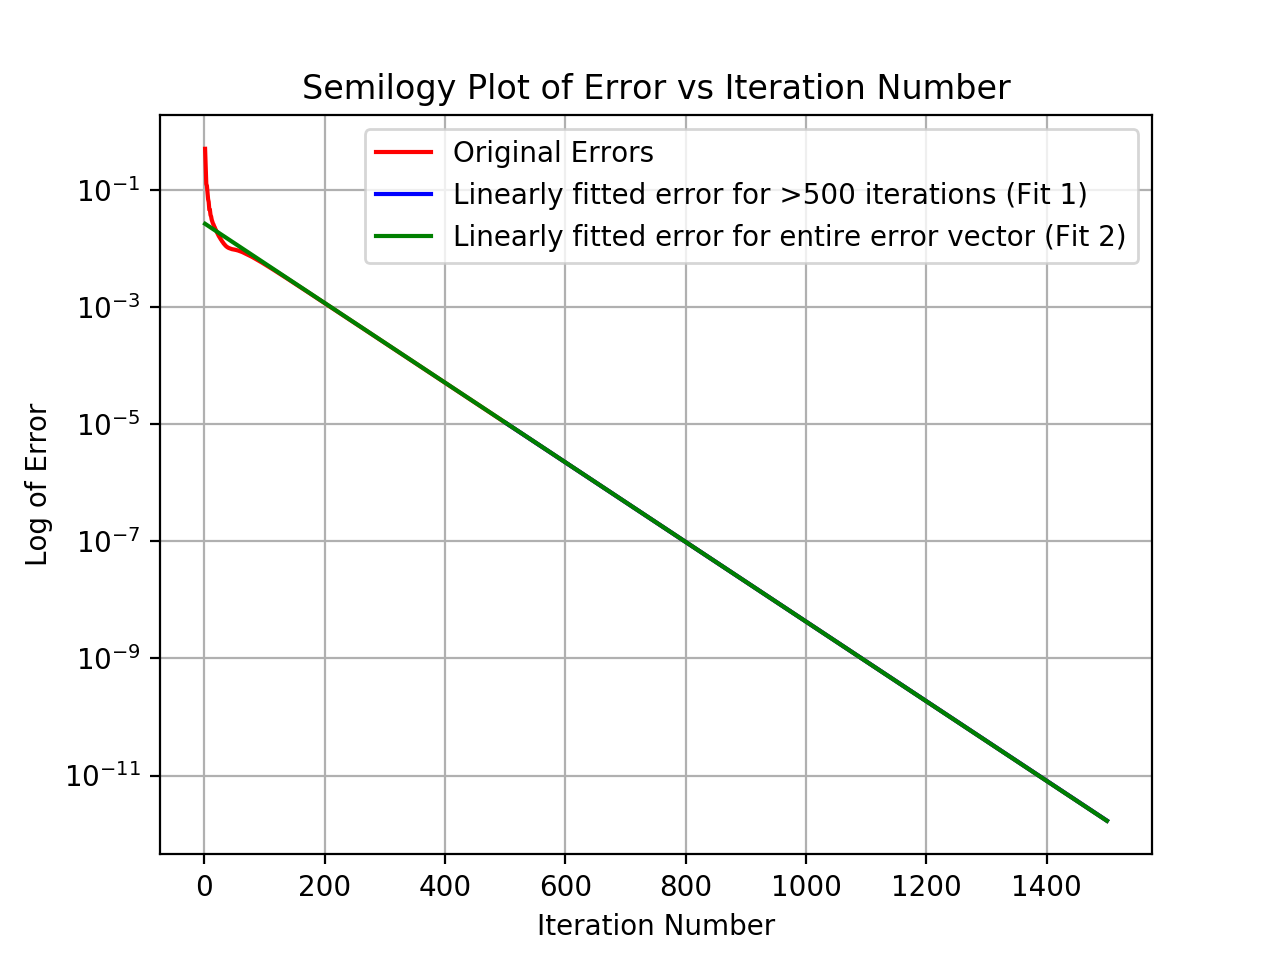
\includegraphics[scale=0.5]{fitting.png}
   	\label{fig:fitting}
   	\caption{Original and fitted Error vs Iteration - Semilog Plot}
\end{figure}

\subsection{Plotting the obtained Potential}
We solved the laplace equation and obtained the potential over the region. We plot it as a 3-D surface plot and contour plot.
\begin{minted}[tabsize = 4]{python3}
fig1 = pl.figure(6)
ax = p3.Axes3D(fig1)
pl.title('The 3-D Surface plot of the potential')
surf = ax.plot_surface(Y,X,Phi,rstride = 1,cstride = 1,
	cmap = matplotlib.cm.viridis,linewidth = 0)
cbaxes = fig1.add_axes([0.96, 0.1, 0.03, 0.8]) 
pl.colorbar(surf,cax = cbaxes,pad = 0.2)
pl.show()

PLOT(x,y,7,"X-axis","Y-axis",pl.contourf,Phi,"Contour Plot of Potential",
	cmap = matplotlib.cm.viridis)
pl.plot(X[X*X + Y*Y < 0.35*0.35],Y[X*X + Y*Y < 0.35*0.35],'ro',
	label = 'Points with potential 1V')
pl.legend()
pl.show()
\end{minted}
\begin{figure}[H]
   	\centering
   	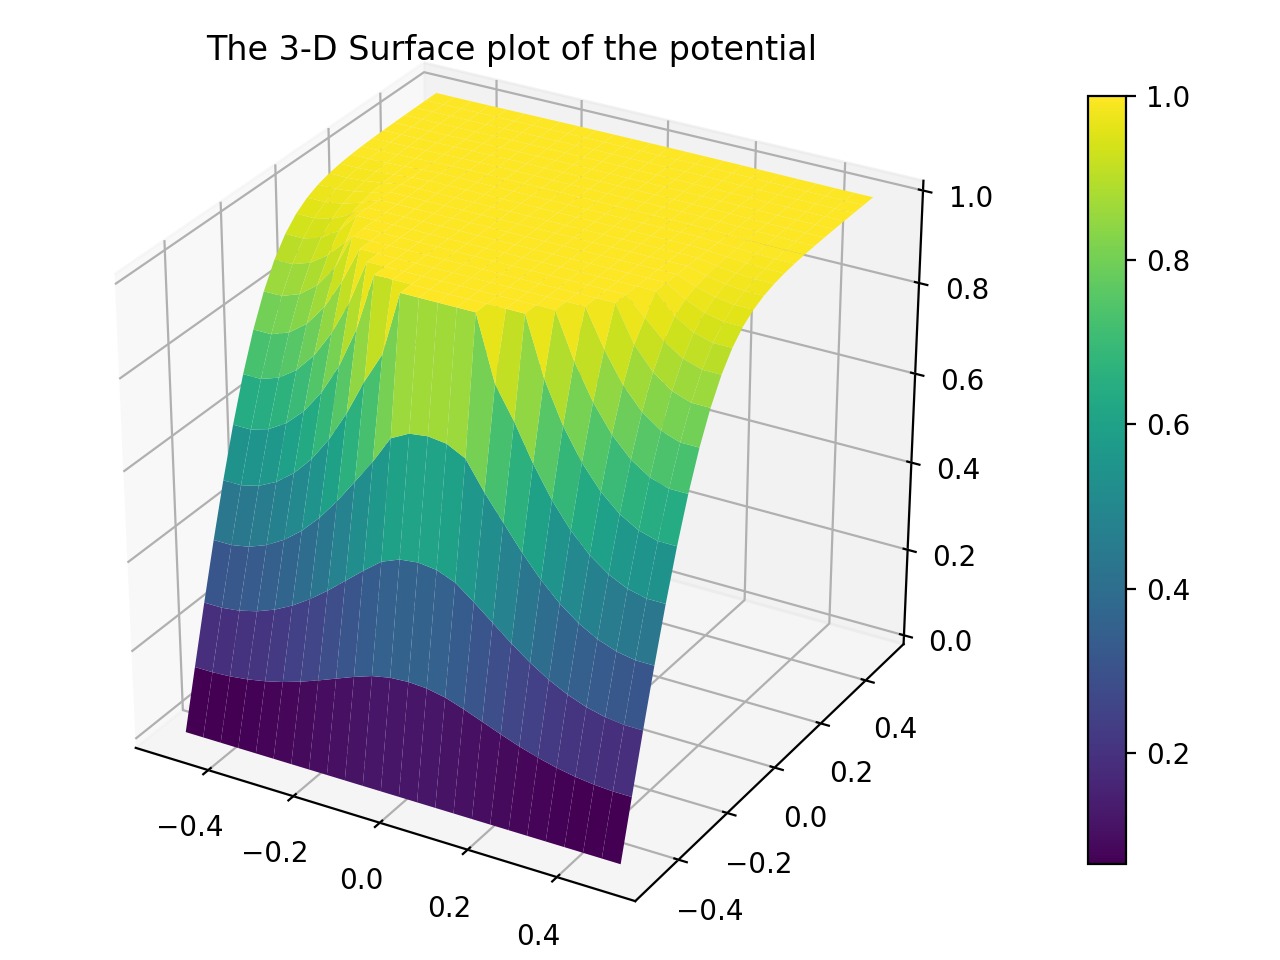
\includegraphics[scale=0.5]{surface_potl.png}
   	\label{fig:3d_potl}
   	\caption{3-D Surface plot of Potential}
\end{figure}
\begin{figure}[H]
   	\centering
   	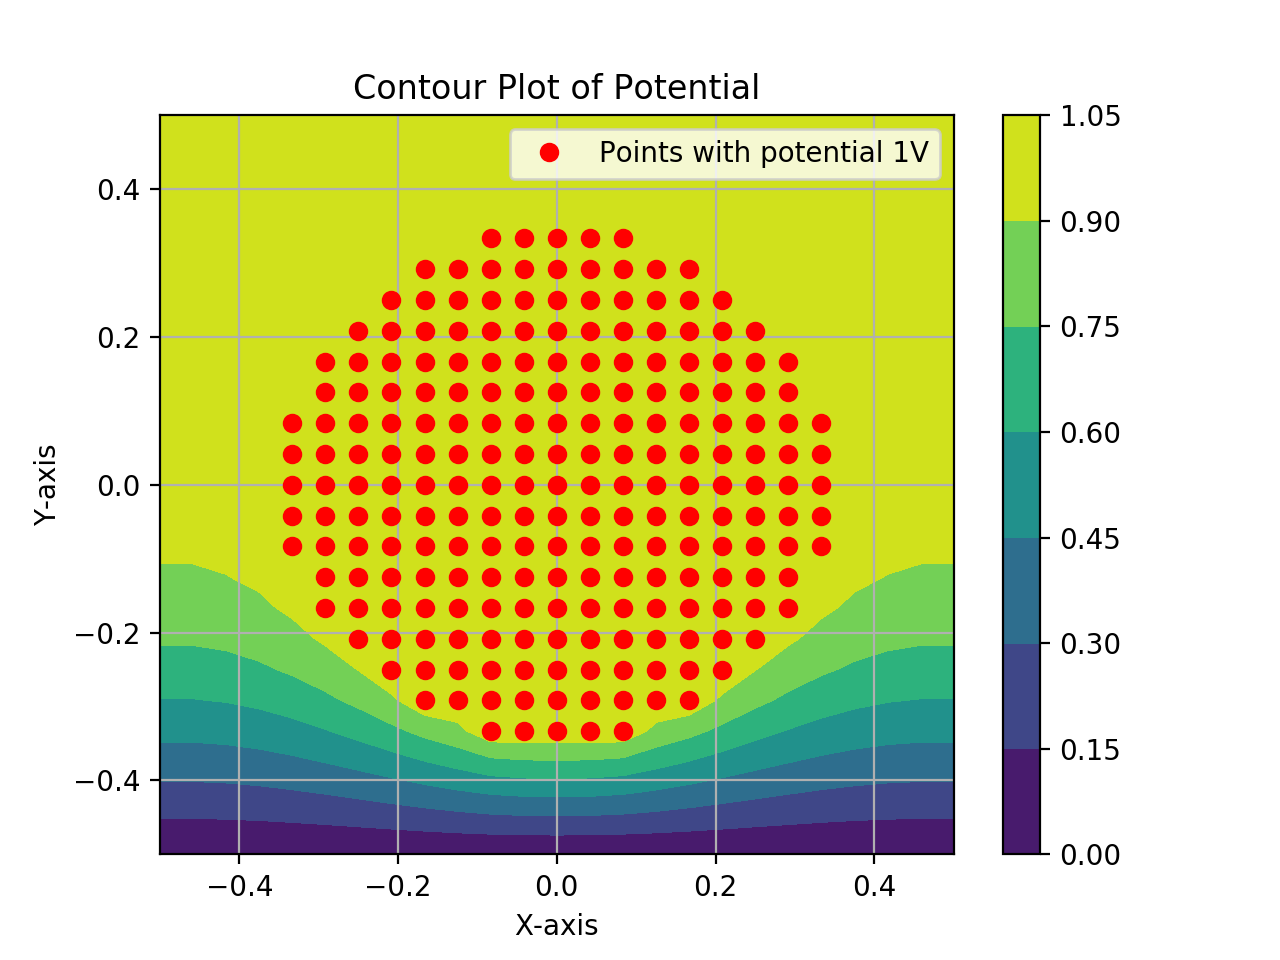
\includegraphics[scale=0.5]{cont_potl_f.png}
   	\label{fig:cont_potl_f}
   	\caption{Contour plot of Potential}
\end{figure}

\subsection{Plotting the Current }
We can calculate the current density from the potential, the relation for which is given by :
\begin{equation}\label{eq:7}
\begin{aligned}
J_x = -\frac{\partial \phi}{\partial x}  \\
J_y = -\frac{\partial \phi}{\partial y}
\end{aligned}
\end{equation}
\begin{equation}\label{eq:8}
\begin{aligned}
J_{x,ij} = -\frac{1}{2} (\phi_{i,j-1} - \phi_{i,j+1}) \\
J_{y,ij} = -\frac{1}{2} (\phi_{i-1,j} - \phi_{i,+1j})
\end{aligned}
\end{equation}
We use quiver plot for highlighting the \textbf{vector quantity} current density's directions.
\begin{minted}[tabsize = 4]{python3}
Jy = pl.zeros((Ny,Nx))
Jx = pl.zeros((Ny,Nx))
Jx[:,1:-1] = 0.5*(Phi[:,0:-2]-Phi[:,2:])
Jy[1:-1,:] = 0.5*(Phi[0:-2,:]-Phi[2:,:])
pl.figure(8)
pl.quiver(x,y,Jx,Jy)
pl.plot(X[X*X + Y*Y < 0.35*0.35],Y[X*X + Y*Y < 0.35*0.35],'ro',
	label = 'Points with potential 1V')
pl.xlabel('X-axis')
pl.ylabel('Y-axis')
pl.legend(loc = 1)
pl.title('Vector plot of current density')
pl.show()
\end{minted}
\begin{figure}[H]
   	\centering
   	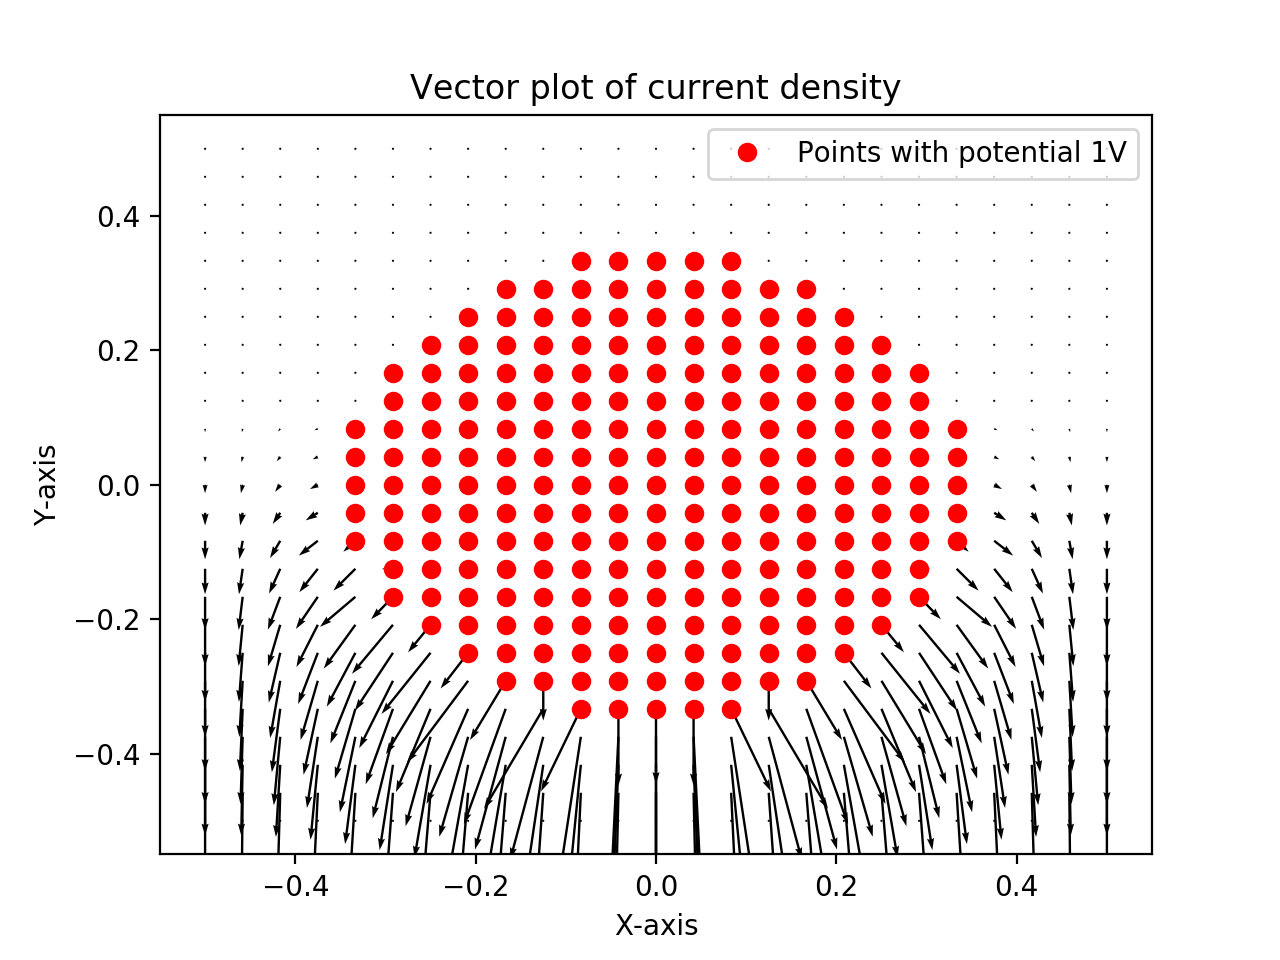
\includegraphics[scale=0.5]{vector_curr.png}
   	\caption{Quiver plot of Current Density}
   	\label{fig:vector_curr}
\end{figure}
We can notice that the current is concentrated in the bottom half between the plate and the ground. This is because of high Electric field in the region between the two compared to other places, which is clear from the Potential contour plot, depicting how rapidly potential varies there. 
\\This is similar to a capacitor under break- down condition. Thus most of the current flows in that region.

\subsection{Calculating Temperature}
The current density and equivalently current, as we saw, is high in the bottom region between plate and ground. Thus there will be more \textbf{ohmic loss} occurring there compared to other places. We, therefore expect that region to heat up strongly and have a higher temperature.
\\
We calculate a 2-D Laplace Equation for Temperature, similar to how we did for Potential in an iterative approach. The Laplace equation for Temperature is given by :
\\
\begin{equation}\label{eq:9}
\nabla . (\kappa \nabla T) = q = \frac{1}{\sigma} |J|^2
\end{equation}
\\
\begin{minted}[tabsize = 4]{python3}
Temp = np.zeros((Ny,Nx))*300
for k in range(Niter):
	Temp[1:-1,1:-1] = 0.25*(Temp[1:-1,0:-2]+Temp[1:-1,2:]+
		Temp[0:-2,1:-1]+Temp[2:,1:-1]+(Jx[1:-1,1:-1]**2)+(Jy[1:-1,1:-1]**2))
	Temp[0,:] = 300
	Temp[1:-1,0] = Temp[1:-1,1]
	Temp[1:-1,-1] = Temp[1:-1,-2]
	Temp[-1,:] = Temp[-2,:]
	Temp[ii] = 300
	
#Contour plot of the Temperature
PLOT(x,y,9,"X-axis","Y-axis",pl.contourf,Temp,
	"Contour Plot of Temperature",cmap = matplotlib.cm.hot)
pl.show()
\end{minted}
\begin{figure}[H]
   	\centering
   	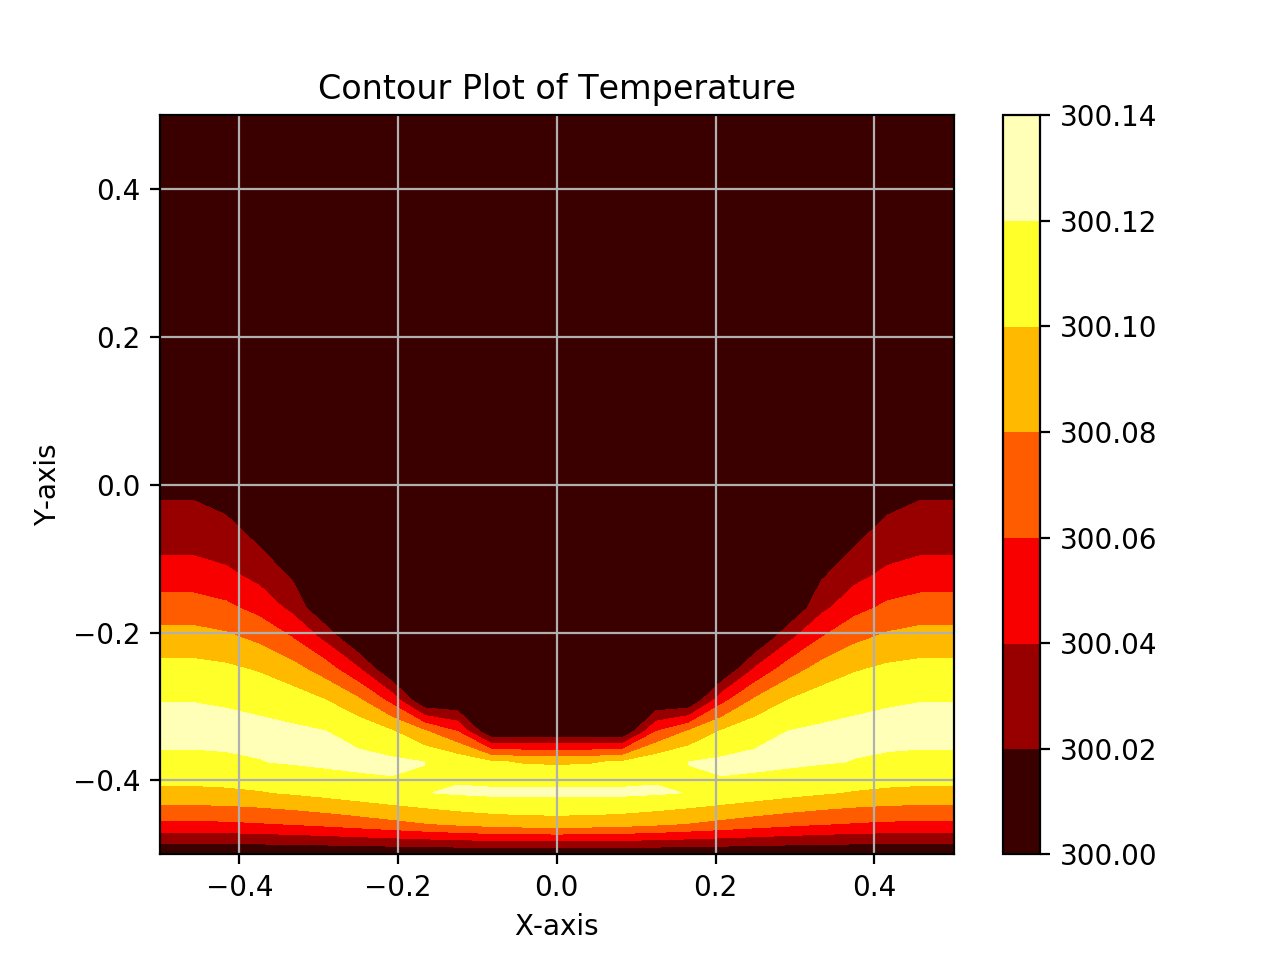
\includegraphics[scale=0.5]{temp.png}
   	\caption{Contour Plot of Temperature}
   	\label{fig:temp}
\end{figure}

\section{Conclusions}
\begin{itemize}
\item We made 2-D contour and 3-D plots for better visual understanding of the physical properties (like Potential, Temperature).
\item We solved 2-D Laplace equation for Potential and Temperature using iterative approach.
\item We used Least Squares Fitting to estimate the parameters of the exponential form of error.
\item We used quiver plot to observe Current density (a vector quantity) over the region.
\item We also quantified the Temperature and analysed the heating effects due to current.
\end{itemize}

\end{document}